\documentclass[10pt,a4paper]{article}
\usepackage[margin=1.7cm]{geometry}
\usepackage[T1]{fontenc}
\usepackage[utf8]{inputenc}
\usepackage[english]{babel}
\usepackage{amsmath,amssymb,booktabs,graphicx,hyperref,array}
\title{Numerical section: Allen--Cahn dynamics and WED minimization}
\author{Reproducible numerical verification}
\date{October 22, 2026}
\begin{document}
\maketitle

\section{Model, discretization, and implementation}
We consider the parabolic system
\begin{align*}
 u_t-\Delta u+u^3-u&=0 &&\text{in }\Omega\times(0,T),\\
 u_{\Gamma,t}-\Delta_\Gamma u_\Gamma+\beta(u_\Gamma^3-u_\Gamma)&=-\partial_nu
 &&\text{on }\Gamma\times(0,T),\\
 u_\Gamma&=u|_\Gamma,
\end{align*}
where $\Omega=(0,2)\times(0,1)$ and $\Gamma=\partial\Omega$. The parameter $\beta>0$ weights the surface reaction potential. The bulk and surface potentials are $F(u)=\frac14(u^2-1)^2$ and $G(u_\Gamma)=\frac{\beta}{4}(u_\Gamma^2-1)^2$, respectively. The energy is
\[
 E(t)=\frac12\int_\Omega|\nabla u|^2+\int_\Omega F(u)
 +\frac12\int_\Gamma|\nabla_\Gamma u_\Gamma|^2+\int_\Gamma G(u_\Gamma).
\]
All variables are dimensionless. OOFEM C++ solves the direct evolution problem. The WED minimizer is a separate Python program that reads the mesh from an OOFEM input, assembles the functional, and is not run by the C++ executable.

The spatial mesh uses bilinear quadrilateral Q1 elements, with a shared scalar field between bulk and boundary, and linear boundary segments. Nine Gauss points are used in quadrilaterals to integrate the Q1 cubic reaction; boundary elements use three Gauss points. The direct solver uses the implicit OOFEM integrator with $\alpha=1$; the MMS time step is $\Delta t=5\,10^{-4}$ with input tolerance $\mathrm{rtol}=10^{-11}$. WED trajectories use piecewise-linear time elements, Gaussian quadrature, a free terminal value, and damped sparse Newton iterations. The rescaled time is $s=t/\varepsilon$, with terminal horizon $S_{\max}$ and physical time step $\Delta t=\varepsilon\Delta s$. The WED tolerance is the infinity norm of the scaled functional gradient; the maximum iteration count is 100.

The nonuniform benchmark uses
\[
 u_0(x,y)=0.2+0.1\left[\cos\!\left(\frac{\pi x}{2}\right)\cos(\pi y)
 +0.25\sin\!\left(\frac{\pi x}{2}\right)\sin(\pi y)\right],
\]
with $\beta=1$ and the manufactured source disabled. The truncated WED functional is
\[
 J_\varepsilon(u)=\int_0^{S_{\max}}e^{-s}\left[\frac12\|u_s\|^2_{L^2(\Omega)\oplus L^2(\Gamma)}
 +\varepsilon\left(\frac12\|\nabla u\|^2_{L^2(\Omega)}+\frac12\|\nabla_\Gamma u_\Gamma\|^2_{L^2(\Gamma)}
 +\int_\Omega F(u)+\int_\Gamma G(u_\Gamma)\right)\right]ds,
\]
subject to $u(0)=u_0$. The implementation minimizes a positively rescaled version of this functional; multiplication by a positive constant does not change its minimizer.

\begin{figure}[ht]\centering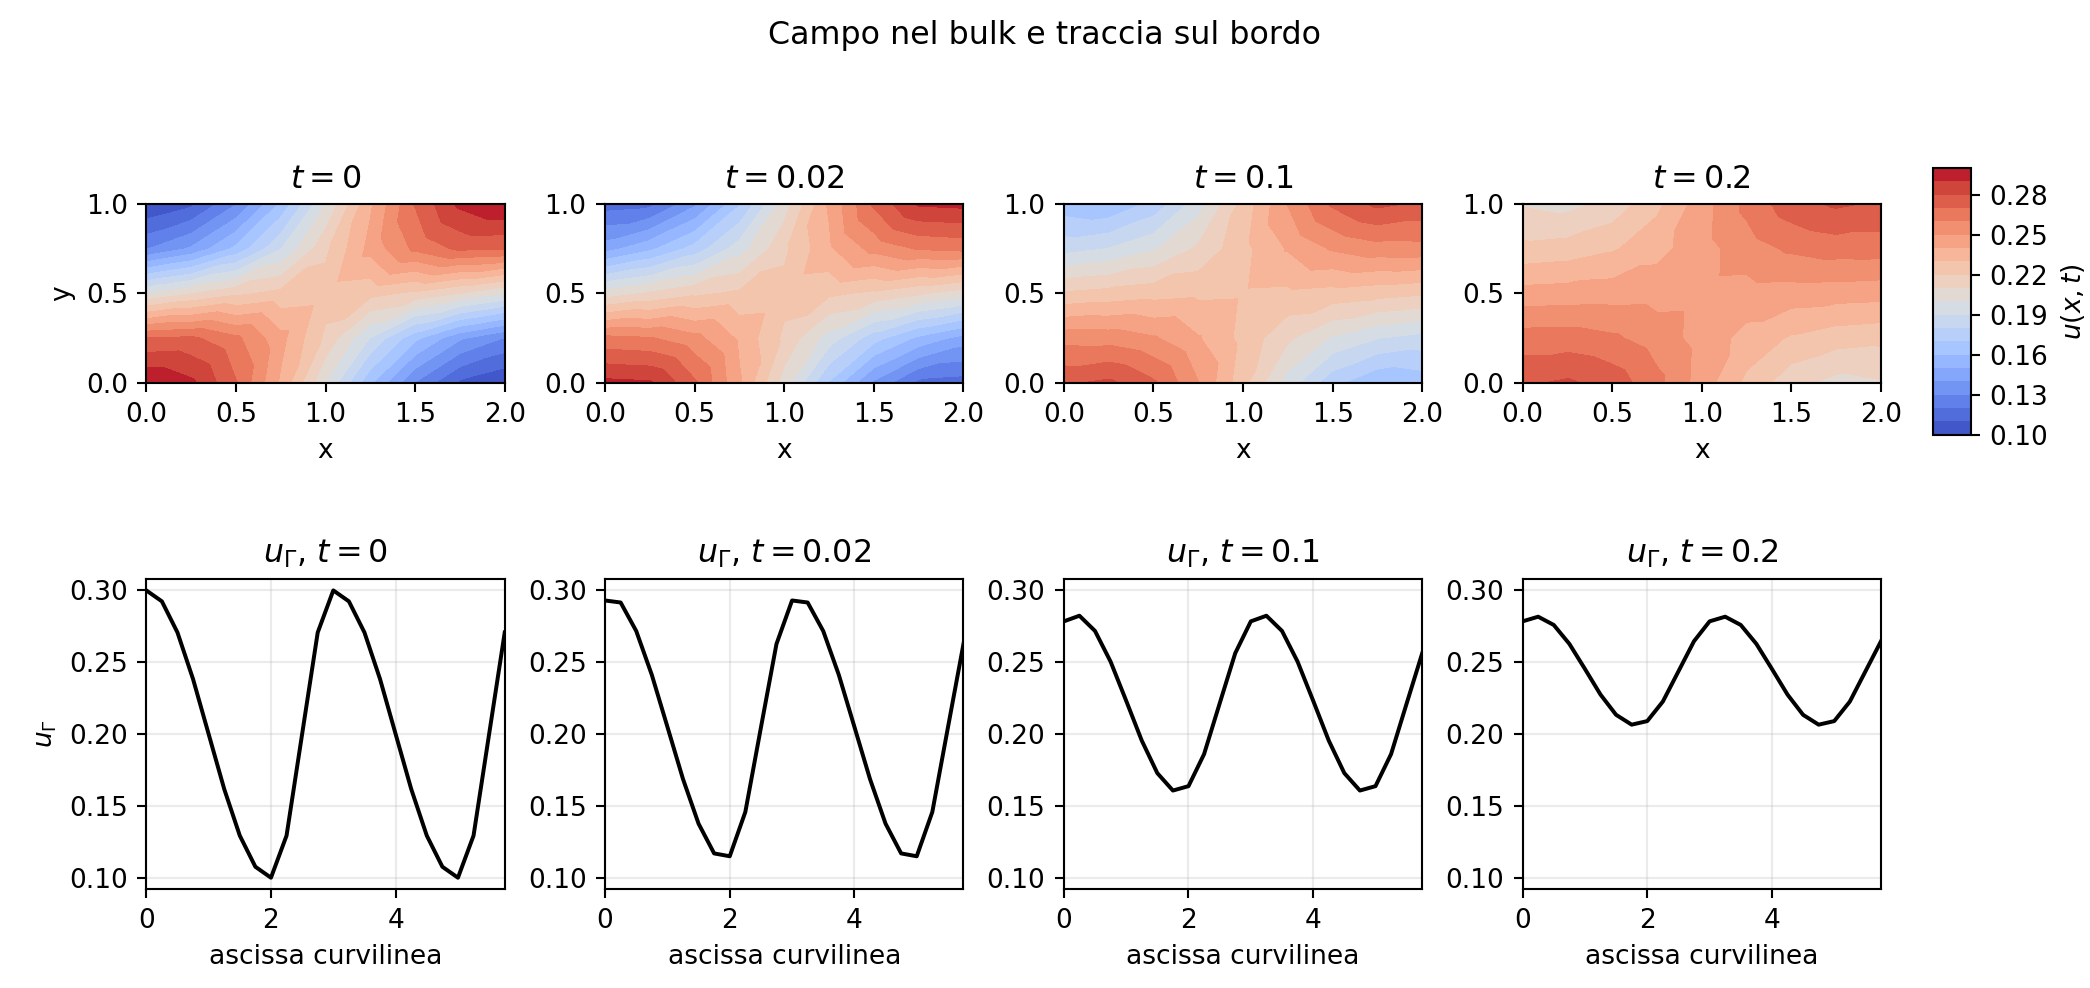
\includegraphics[width=.96\linewidth]{paper_figures/figure1_field_boundary.png}\caption{Bulk field snapshots and boundary trace at $t=0,0.02,0.1,0.2$ for the nonuniform benchmark on $[0,2]\times[0,1]$, an $8\times4$ mesh, disabled manufactured source, and $\beta=1$.}\label{fig:field}\end{figure}

\section{Direct solver verification: manufactured solution}
The manufactured solution is
\[
 u^*(x,y,t)=0.2+0.1e^{-t}\left[\cos\!\left(\frac{\pi x}{2}\right)\cos(\pi y)
 +0.25\sin\!\left(\frac{\pi x}{2}\right)\sin(\pi y)\right],
\]
with consistent bulk and surface sources and $\beta=1$. We report the nodal RMS error at $T=0.02$; $h$ denotes the quadrilateral cell width. The observed slope $p=\log_2(e_h/e_{h/2})$ is empirical.
\begin{center}\small
\begin{tabular}{rrrrrrr}
\toprule
mesh & nodes/DoFs & $h$ & nodal RMS & maximum absolute & $\Delta t$ & $p$\\
\midrule
$8\times4$ &45&0.250&$7.8821\,10^{-5}$&$1.8014\,10^{-4}$&$5\,10^{-4}$&--\\
$16\times8$&153&0.125&$1.7886\,10^{-5}$&$3.8000\,10^{-5}$&$5\,10^{-4}$&2.140\\
$32\times16$&561&0.0625&$4.3869\,10^{-6}$&$9.4361\,10^{-6}$&$5\,10^{-4}$&2.028\\
\bottomrule
\end{tabular}
\end{center}
The nodal RMS is $[N^{-1}\sum_{i=1}^N(u_i-u_i^*)^2]^{1/2}$. The observed convergence is consistent with second-order spatial accuracy for this direct-solver MMS case; it does not verify the WED minimizer.

\section{Dissipation and discrete energy balance}
We define bulk and surface dissipation by
\[
 D_\Omega=\int_0^T\!\int_\Omega|u_t|^2,\qquad
 D_\Gamma=\int_0^T\!\int_\Gamma|u_{\Gamma,t}|^2,
\]
and the residual by $R_E=E(T)-E(0)+D_\Omega+D_\Gamma$. The postprocessing approximates $u_t$ by backward differences and evaluates dissipation with FEM mass matrices. The runs use $T=0.1$, domain $[0,1]^2$, a $20\times20$ quadrilateral mesh, $u_0(x,y)=0.1+0.05\cos(2\pi x)$, $\beta=1$, and no manufactured source; only the time step changes. This is a finite-step discrete check, not an analytical stability proof.
\begin{center}\small
\begin{tabular}{rrrrrrr}
\toprule
$\Delta t$&$E(0)$&$E(T)$&$D_\Omega$&$D_\Gamma$&$R_E$&$|R_E|/E(0)$\\
\midrule
0.00500&1.284456&1.209120&0.022138&0.047763&$-5.4350\,10^{-3}$&0.004231\\
0.00250&1.284456&1.209018&0.022887&0.049612&$-2.9395\,10^{-3}$&0.002289\\
0.00125&1.284456&1.208967&0.023310&0.050636&$-1.5420\,10^{-3}$&0.001201\\
\bottomrule
\end{tabular}
\end{center}
The residual is negative and its normalized magnitude decreases from $0.423\%$ to $0.120\%$ as the time step is refined. Since the dissipation is numerically approximated, the finite-step residual is not expected to vanish exactly. Figure~\ref{fig:energy} shows the bulk and surface energies and their sum; monotonicity is not required of the separate components.

\section{The $\varepsilon\to0$ limit for WED minimizers}
We compare space--time $L^2$ errors with the direct OOFEM trajectory on the same $8\times4$ mesh, interpolating both solutions over the common physical window $t\in[0,0.1]$. Define
\[
 E_\Omega=\left(\int_0^{0.1}\|u_{\rm WED}(t)-u_{\rm OOFEM}(t)\|^2_{L^2(\Omega)}dt\right)^{1/2},\quad
 E_\Gamma=\left(\int_0^{0.1}\|u_{\Gamma,\rm WED}(t)-u_{\Gamma,\rm OOFEM}(t)\|^2_{L^2(\Gamma)}dt\right)^{1/2}.
\]
The direct reference uses $\Delta t=0.001$. In the first series, $S_{\max}=12$, $\Delta s=0.1$, and WED tolerance $2\,10^{-5}$ are fixed, so the physical step changes as $\Delta t=\varepsilon\Delta s$. In the second series, $\Delta t=0.005$ is fixed and $\Delta s=0.005/\varepsilon$; hence $S_{\max}$ and the tolerance are unchanged, while the resolution in $s$ changes. Each minimization converges in two Newton iterations.
\begin{center}\small
\begin{tabular}{rrrrrrr}
\toprule
series&$\varepsilon$&$\Delta s$&$\Delta t$&$\varepsilon S_{\max}$&$E_\Omega$&$E_\Gamma$\\
\midrule
fixed $\Delta s$&0.1000&0.100&0.0100&1.200&$1.8485\,10^{-3}$&$3.1960\,10^{-3}$\\
&0.0500&0.100&0.0050&0.600&$1.1511\,10^{-3}$&$2.0198\,10^{-3}$\\
&0.0250&0.100&0.0025&0.300&$6.8730\,10^{-4}$&$1.1978\,10^{-3}$\\
&0.0125&0.100&0.00125&0.150&$3.8735\,10^{-4}$&$6.6759\,10^{-4}$\\
fixed $\Delta t$&0.1000&0.050&0.0050&1.200&$1.8475\,10^{-3}$&$3.1947\,10^{-3}$\\
&0.0500&0.100&0.0050&0.600&$1.1511\,10^{-3}$&$2.0198\,10^{-3}$\\
&0.0250&0.200&0.0050&0.300&$6.8614\,10^{-4}$&$1.1959\,10^{-3}$\\
&0.0125&0.400&0.0050&0.150&$3.8299\,10^{-4}$&$6.6022\,10^{-4}$\\
\bottomrule
\end{tabular}
\end{center}
The local slope $p=\log(E_\varepsilon/E_{\varepsilon/2})/\log 2$ is empirical, not a theoretical order. For fixed $\Delta s$, the bulk/surface slopes are 0.68/0.66, 0.74/0.75, and 0.83/0.84; with fixed physical $\Delta t$, they are approximately 0.68/0.66, 0.75/0.76, and 0.84/0.86. The decreasing trend is similar in both protocols. Fixing physical $\Delta t$ reduces temporal-step confounding but does not eliminate all time-discretization error; at $\varepsilon=0.0125$ it gives $\Delta s=0.4$.

For this smallest $\varepsilon$, we additionally halve $\Delta s$ from 0.4 to 0.2 while keeping $S_{\max}=12$, mesh, and tolerance $2\,10^{-5}$ fixed. Both runs take two Newton iterations. Errors against OOFEM change by about $0.9\%$ in bulk and on the boundary; the difference between WED trajectories is much smaller than the total error:
\begin{center}\small
\begin{tabular}{rrrrrr}
\toprule
$\Delta s$&$\Delta t=\varepsilon\Delta s$&iterations&$E_\Omega$ vs OOFEM&$E_\Gamma$ vs OOFEM&WED path difference, bulk/surface\\
\midrule
0.4&0.0050&2&$3.82985\,10^{-4}$&$6.60221\,10^{-4}$&reference\\
0.2&0.0025&2&$3.86483\,10^{-4}$&$6.66145\,10^{-4}$&$4.16\,10^{-6}/6.44\,10^{-6}$\\
\bottomrule
\end{tabular}
\end{center}
The $\varepsilon$ trend is stable under this targeted time-step check, although the error against OOFEM does not decrease monotonically when only the time step is refined. The slopes are therefore not interpreted as asymptotic method orders.
\begin{figure}[ht]\centering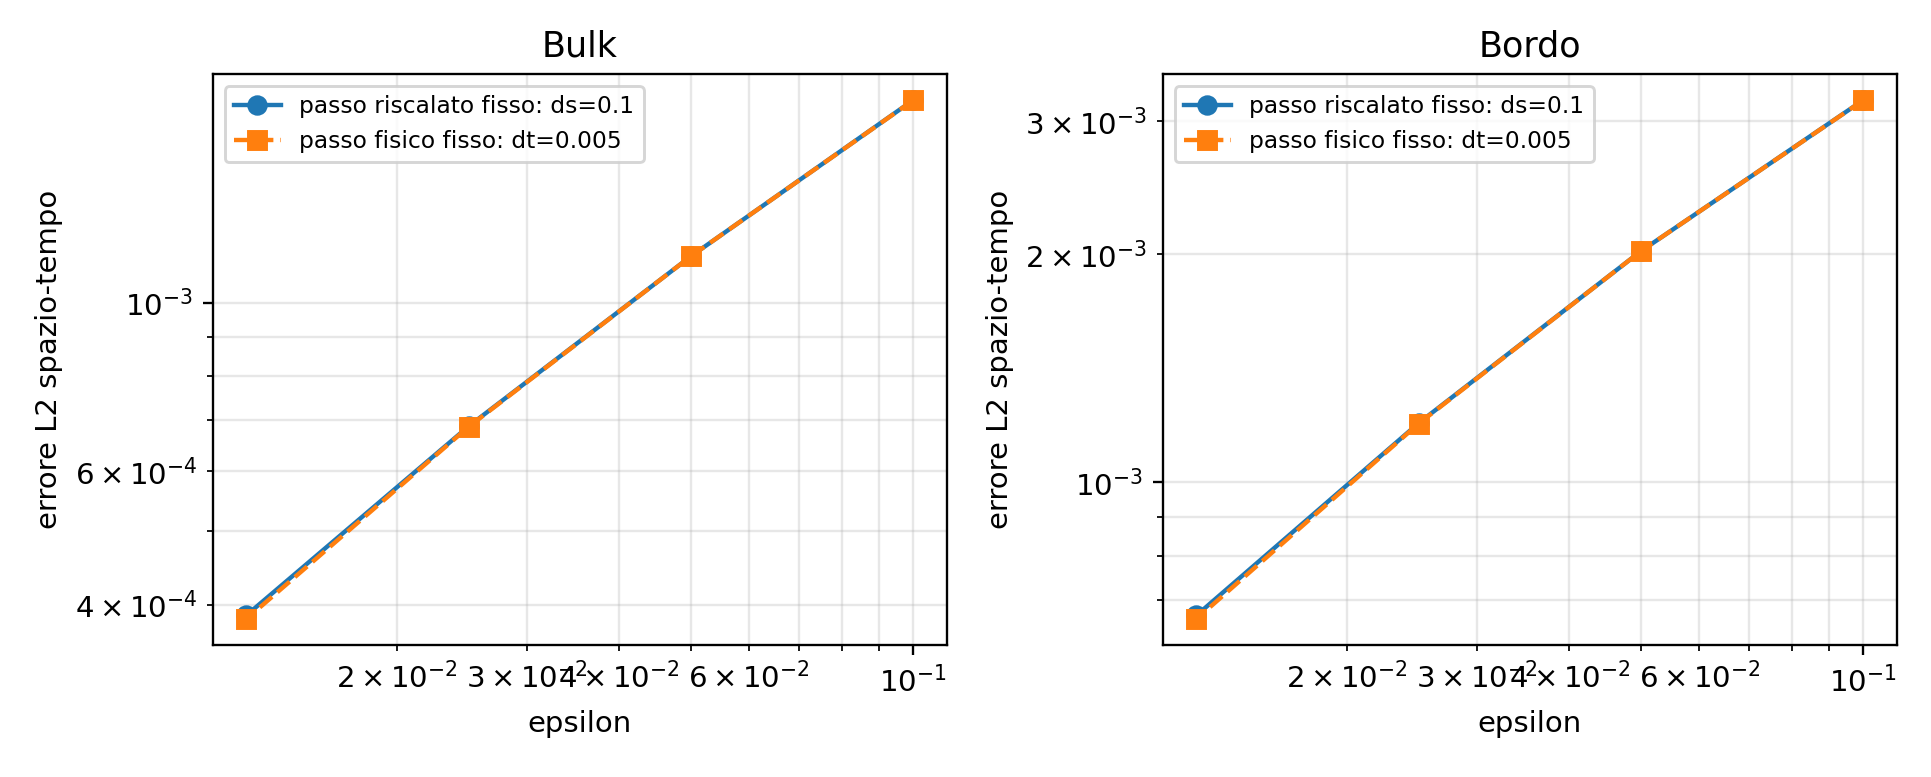
\includegraphics[width=.96\linewidth]{paper_figures/figure2_epsilon.png}\caption{Bulk and boundary errors versus $\varepsilon$. Solid lines: fixed $\Delta s=0.1$; dashed lines: fixed physical $\Delta t=0.005$. Each error is integrated on $[0,0.1]$ against the direct OOFEM trajectory ($\Delta t=0.001$).}\label{fig:epsilon}\end{figure}

\section{WED horizon sensitivity and spatial convergence}
\subsection{Truncated horizon}
With $\varepsilon=0.05$, $\Delta s=0.1$, tolerance $2\,10^{-5}$, and an $8\times4$ mesh, we compare $S_{\max}=6,12$ with 18 over $t\in[0,0.1]$. The space--time RMS is computed over nodes as $[\int_0^{0.1}N^{-1}\sum_i|u_i^{S_{\max}}(t)-u_i^{18}(t)|^2dt]^{1/2}$; the maximum is the largest nodal difference over the same interval.
\begin{center}\small
\begin{tabular}{rrrr}
\toprule
$S_{\max}$&$\Delta t=\varepsilon\Delta s$&RMS vs $S_{\max}=18$&maximum nodal difference\\
\midrule
6&0.005&$3.6689\,10^{-5}$&$3.0215\,10^{-4}$\\
12&0.005&$1.5575\,10^{-7}$&$1.1327\,10^{-6}$\\
18&0.005&0 (reference)&0 (reference)\\
\bottomrule
\end{tabular}
\end{center}
This is a truncation-sensitivity test for the selected initial data and comparison window, not a uniform estimate for other cases.
\begin{figure}[ht]\centering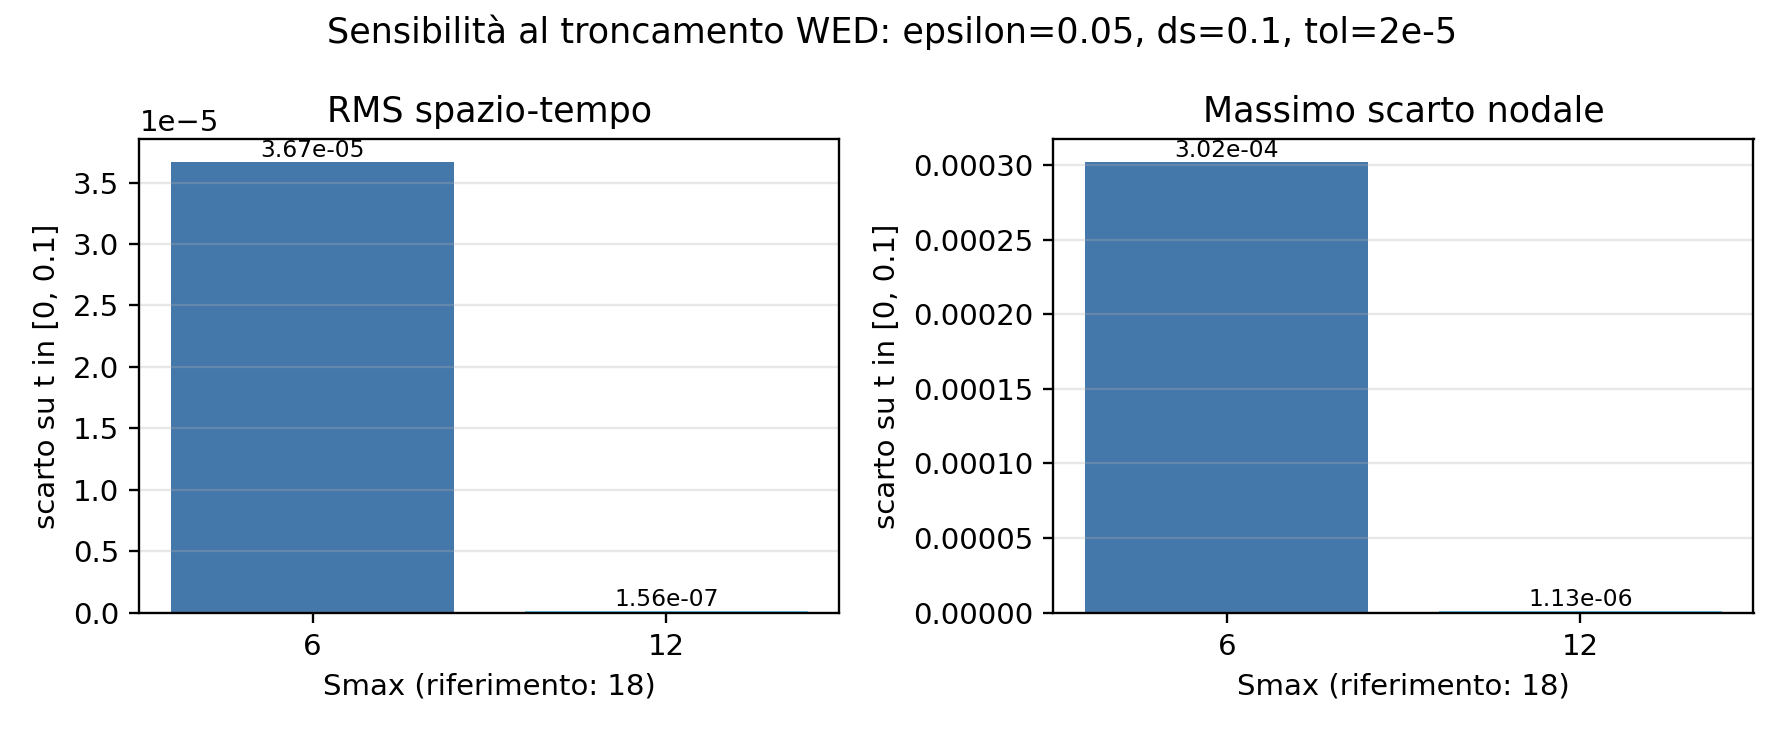
\includegraphics[width=.78\linewidth]{paper_figures/figure3_horizon.png}\caption{RMS and maximum nodal differences relative to $S_{\max}=18$, for $\varepsilon=0.05$, $\Delta s=0.1$, and $t\in[0,0.1]$.}\label{fig:horizon}\end{figure}

\subsection{Mesh refinement}
WED trajectories at $\varepsilon=0.05$ are compared with the $32\times16$ WED solution as a numerical reference. Space--time norms are evaluated on $t\in[0,0.1]$. The baseline uses $\Delta s=0.1$, tolerance $2\,10^{-5}$; the refinement check uses $\Delta s=0.05$, tolerance $2\,10^{-6}$. The fine mesh is not an exact solution. The table reports errors against the reference and empirical bulk/surface slopes estimated from the two coarse meshes.
\begin{center}\scriptsize
\begin{tabular}{llrrrrr}
\toprule
run&mesh&$h$&$E_\Omega$&$E_\Gamma$&$p_\Omega$&$p_\Gamma$\\
\midrule
baseline&$8\times4$&0.250&$2.1961\,10^{-4}$&$3.1175\,10^{-4}$&2.107&2.243\\
&$16\times8$&0.125&$5.0963\,10^{-5}$&$6.5835\,10^{-5}$&--&--\\
&$32\times16$&0.0625&0 (ref.)&0 (ref.)&--&--\\
refined&$8\times4$&0.250&$2.1977\,10^{-4}$&$3.0581\,10^{-4}$&2.108&2.216\\
&$16\times8$&0.125&$5.0972\,10^{-5}$&$6.5840\,10^{-5}$&--&--\\
&$32\times16$&0.0625&0 (ref.)&0 (ref.)&--&--\\
\bottomrule
\end{tabular}
\end{center}
The estimated order changes by about 0.001 in the bulk and 0.028 on the boundary between settings. For these grids the trend is consistent with second-order spatial convergence and is stable under the time-step and stopping-tolerance refinement. WED/OOFEM differences include the finite-$\varepsilon$ bias and are not used to infer spatial order.
\begin{figure}[ht]\centering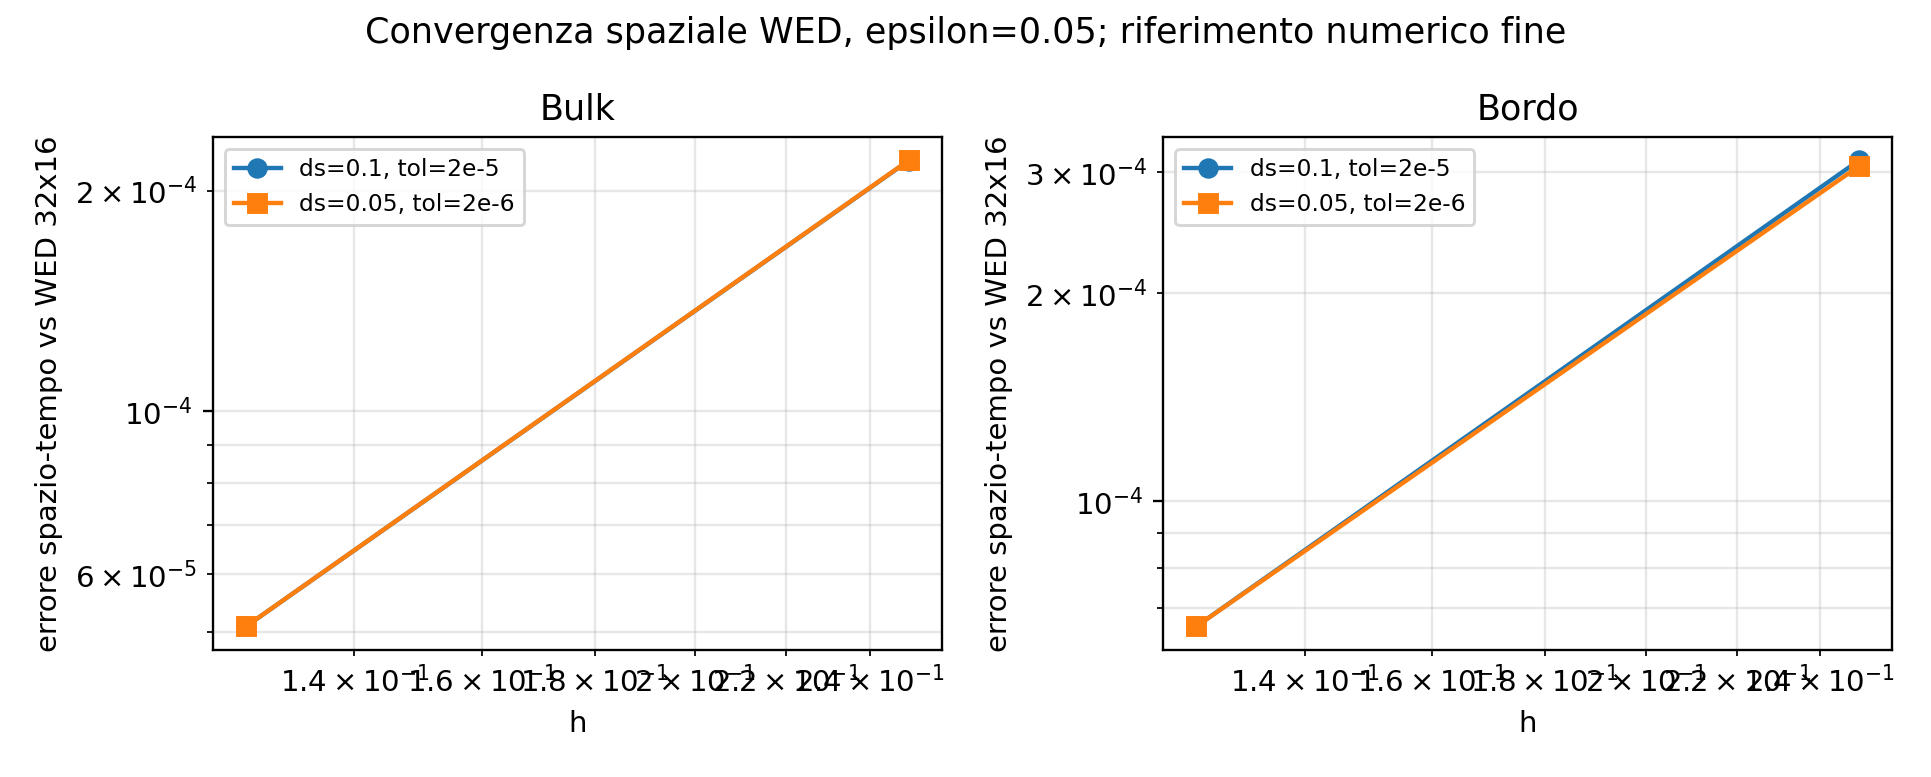
\includegraphics[width=.96\linewidth]{paper_figures/figure4_mesh.png}\caption{Bulk and surface errors against the $32\times16$ WED trajectory at fixed $\varepsilon$. The fine-grid path is a numerical reference; the two series use the time steps and tolerances listed in the legend.}\label{fig:mesh}\end{figure}
\begin{figure}[ht]\centering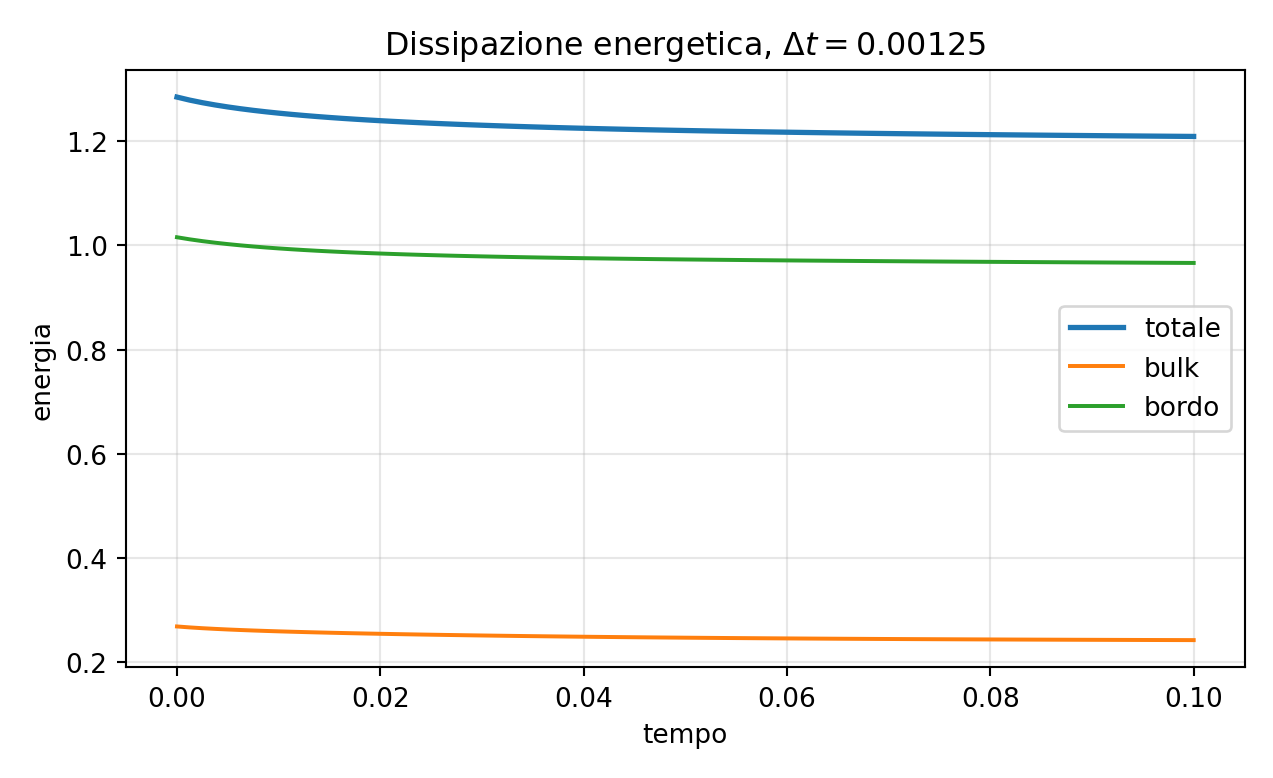
\includegraphics[width=.78\linewidth]{paper_figures/figure5_energy.png}\caption{Bulk, surface, and total energy for direct Allen--Cahn evolution on $[0,1]^2$, a $20\times20$ quadrilateral mesh, $T=0.1$, $\Delta t=0.00125$, and $\beta=1$. Total energy decreases; monotonicity is not assumed for the separate components.}\label{fig:energy}\end{figure}

\section{Effect of the surface parameter $\beta$}
We vary $\beta\in\{0.5,1,2,5\}$ while keeping the domain $[0,2]\times[0,1]$, $8\times4$ mesh, nonuniform initial data defined above, and disabled manufactured source fixed. The direct OOFEM series uses $\Delta t=5\,10^{-4}$ until $T=0.02$; WED uses $\varepsilon=0.05$, $S_{\max}=4$, $\Delta s=0.1$, tolerance $2\,10^{-5}$ until $T=0.2$. Since the final times differ, the series are shown separately and are not compared pointwise. $M_\Gamma(T)=|\Gamma|^{-1}\int_\Gamma u_\Gamma(T)$ is the boundary mean.
\begin{center}\small
\begin{tabular}{rrrrrr}
\toprule
backend, $T$&$\beta$&$M_\Gamma(T)$&$E_\Gamma(T)$&$D_\Omega$&$D_\Gamma$\\
\midrule
OOFEM, 0.02&0.5&0.202747&0.739877&0.005098&0.018408\\
&1&0.204470&1.423137&0.005238&0.020230\\
&2&0.207956&2.783037&0.006023&0.029831\\
&5&0.218748&6.806088&0.012690&0.109610\\
WED, 0.2&0.5&0.220390&--&--&--\\
&1&0.233905&--&--&--\\
&2&0.264304&--&--&--\\
&5&0.382729&--&--&--\\
\bottomrule
\end{tabular}
\end{center}
The listed surface energies and dissipations are computed for the direct transient; they are not reported for WED here. A response to $\beta$ is observed for this initial condition, without claiming universal monotonicity or a relaxation time.
\begin{figure}[ht]\centering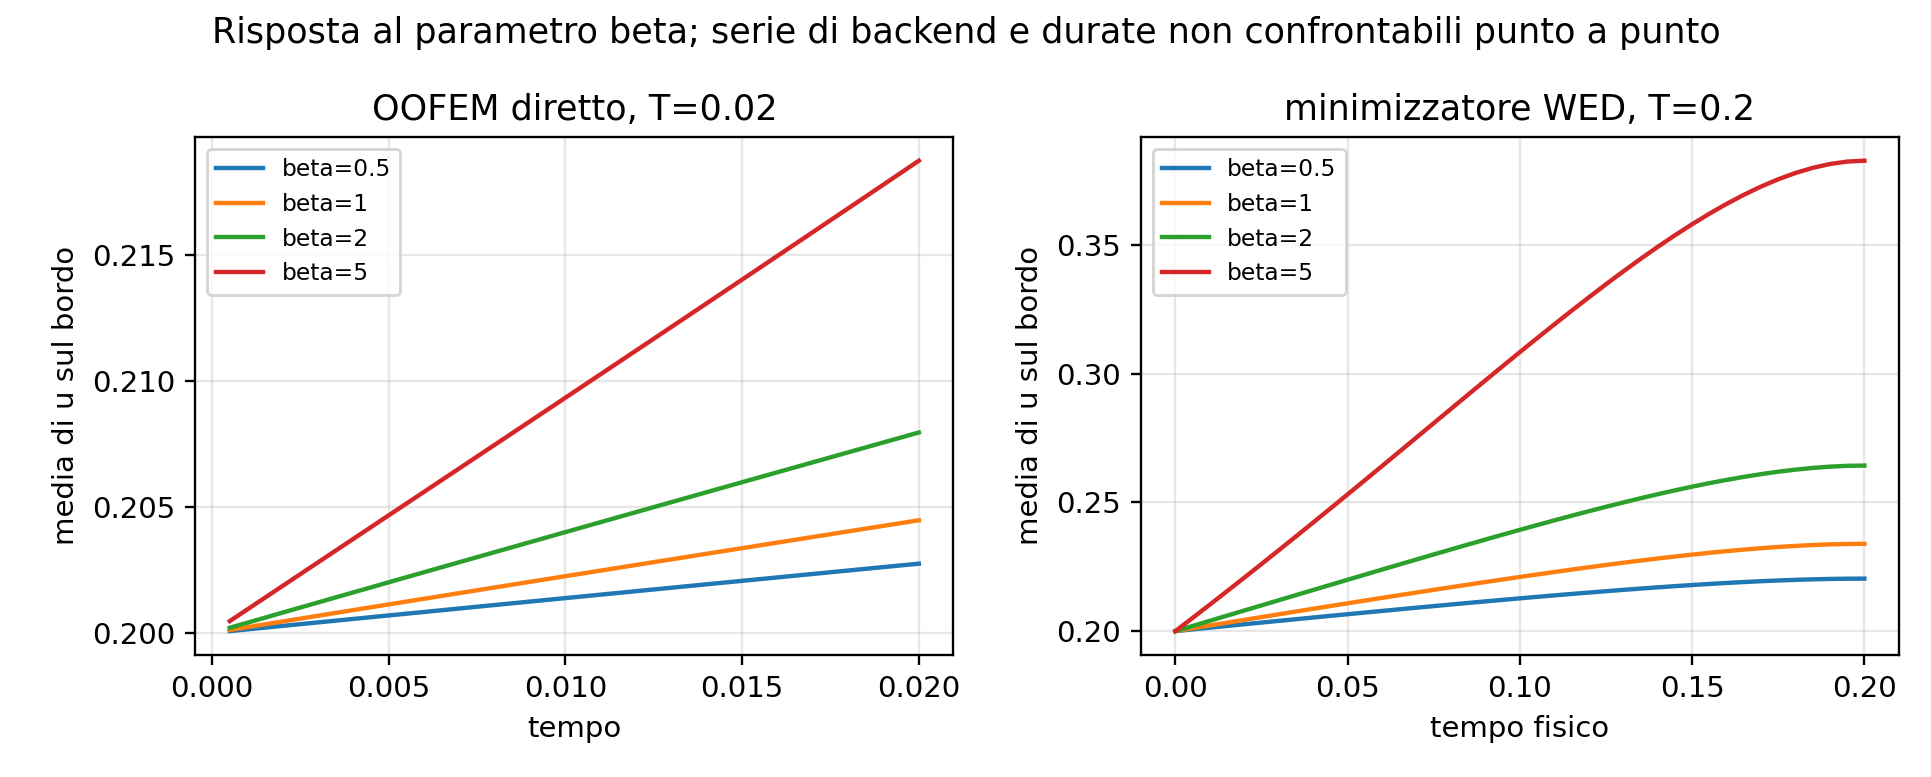
\includegraphics[width=.96\linewidth]{paper_figures/figure6_beta.png}\caption{Boundary mean for $\beta=0.5,1,2,5$. Left: direct OOFEM through $T=0.02$, $\Delta t=5\,10^{-4}$. Right: WED minimizer through $T=0.2$, $\varepsilon=0.05$, $S_{\max}=4$, $\Delta s=0.1$. Backend and final time differ between panels.}\label{fig:beta}\end{figure}

\section{Limitations and reproducibility}
The study is two-dimensional, parabolic, and uses quadrilateral Q1 elements. The triangular P1 benchmark and hyperbolic wave variant are outside scope. MMS and energy-balance checks verify the direct solver, not the WED minimizer; the $\varepsilon$, horizon, and mesh studies concern the separate WED backend. Reported orders are empirical for the stated benchmarks. WED/OOFEM differences include finite-$\varepsilon$ bias and are not used as mesh-convergence evidence.

Reproduction inputs, logs, CSV data, and scripts are archived in \texttt{doc/stvowu\_validation}; commands, dependencies, and result-to-driver mappings are documented in the README. The energy check uses backward differences on saved fields. Conclusions are limited to the reported data, meshes, and parameters and do not constitute universal validation.
\end{document}
